\documentclass[9pt,hyperref={pdfpagelabels=false},xcolor=table]{beamer}
\usepackage{multicol}

% Contact information: 
%   Jorge M. Cruz-Duarte (jorge.cruz@tec.mx)
%   Nov. 29, 2019

\usepackage{lmodern, ragged2e, CJKutf8, booktabs, subfig,adjustbox, graphicx, amsmath, amssymb, amsthm, amsfonts, mathtools, multirow,wrapfig,lipsum,tikz, tikz-cd,tikz-3dplot,pgfplots}
\usetikzlibrary{shapes.geometric}
% \usepackage{amsmath, amsthm, amssymb, amsfonts, amsthm, bbold, bm}
\usepackage[alpine,misc,geometry,electronic]{ifsym}
\usepackage[style=phys]{biblatex}
\usepackage[lined,boxed,vlined,ruled,linesnumbered]{algorithm2e}
\SetKw{Continue}{continue}
\SetKw{Or}{or}
\SetKw{Until}{until}
\addbibresource{bibliography.bib}
\renewcommand{\footnotesize}{\tiny}
\newcommand{\norm}[1]{\left\lVert#1\right\rVert}
\makeatletter
\@newctr{footnote}[page]
\makeatother

\usetheme{CambridgeUS}
\renewcommand{\raggedright}{\leftskip=0pt \rightskip=0pt plus 0cm}

\definecolor{UQPurple}{RGB}{0, 32, 159}
% This is the trademark pruple that UQ uses
\definecolor{UQPurple}{RGB}{81,36,122}
\newcommand{\hl}[1]{{\textcolor{UQPurple}{#1}}}

% Theme setup
\titlegraphic{\includegraphics[scale=0.05]{img/UQ_color_logo.png}}

% \makeatletter
\setbeamertemplate{headline}{%
  \leavevmode%
  \hbox{%
    \begin{beamercolorbox}[wd=\paperwidth,ht=2.5ex,dp=1.125ex]{palette quaternary}%
      \insertsectionnavigationhorizontal{\paperwidth}{}{\hskip0pt plus1filll}
    \end{beamercolorbox}%
  }
}
\setbeamertemplate{footline}{\hspace*{2ex} \insertshortauthor \hfill \textcolor{UQPurple}{\insertshorttitle} \hfill \textbf{\insertframenumber{}} / \inserttotalframenumber \hspace*{2ex}}

\setbeamercolor{item projected}{bg=UQPurple}
\setbeamertemplate{enumerate items}[default]
\setbeamercolor*{enumerate item}{fg=UQPurple}

\setbeamertemplate{navigation symbols}{}
% \setbeamertemplate{footline}[\insertshorttitle frame number]
\setbeamertemplate{bibliography item}[text]
\setbeamertemplate{theorems}[numbered]

\setbeamerfont{title}{series = \bfseries, parent = structure}
\setbeamerfont{frametitle}{series = \bfseries, parent = structure}
\setbeamerfont{headline}{series = \bfseries, size = \tiny, parent = structure}

\setbeamercolor{title}{fg = white, bg = UQPurple}
\setbeamercolor{frametitle}{fg = white, bg = UQPurple}
\setbeamercolor{structure}{fg = UQPurple}
\setbeamercolor{section in head/foot}{fg = black, bg = UQPurple!40}
\setbeamercolor{subsection in head/foot}{fg = black, bg = UQPurple!20}

\setbeamercolor{block title}{use=structure,fg=white,bg=structure.fg!75!black}
\setbeamercolor{block body}{parent=normal text,use=block title,bg=UQPurple!20} %block title.bg!10!bg}
\makeatletter
\def\th@mystyle{%
  \normalfont % body font
  \setbeamercolor{block title example}{bg=orange,fg=white}
  \setbeamercolor{block body example}{bg=orange!20,fg=black}
  \def\inserttheoremblockenv{exampleblock}
}
\makeatother
\theoremstyle{mystyle}
\newtheorem*{remark}{Remark}

\usepackage{tikz,color,xcolor,amsmath,amsfonts,stmaryrd,amssymb,bm}
\usepackage{url}

%Just having a look at what it looks like without it
\setbeamertemplate{background}{\tikz[overlay,remember picture]\node[opacity=0.07]at (current page.center){\includegraphics[width=6cm]{img/UQ_purple_logo.png}};}


\newcommand{\maketitleandtoc}{%
  {%
      \setbeamertemplate{headline}{}%
      \setbeamertemplate{footline}{}%
      \begin{frame}[noframenumbering]%
        \titlepage%
      \end{frame}%
      \begin{frame}[noframenumbering]%
        \frametitle{Outline}%
        \tableofcontents%
      \end{frame}%
    }}

\newcommand{\noheadfoot}[1]{%
  {%
      \setbeamertemplate{headline}{}%
      \setbeamertemplate{footline}{}%
      {#1}
    }
}

\title{Optimizing Gaussian Processes}  
\author[Michael Ciccotosto-Camp]{{\bf Honours Research Project}} 
%\institute{}
\date{
Michael Ciccotosto-Camp - 44302913 \\
}

\begin{document}

\maketitle

\section{The Kernel Trick}

\begin{frame}
    \frametitle{Problem Setting and Motivation}
    \begin{itemize}
        \item Suppose we have some inputs $\left[ \text{\PaperPortrait}_1 , \ldots , \text{\PaperPortrait}_n \right]$ (with their corressponding experimental observations $\left[ y_1 , \ldots , y_n \right]$), where $\text{\PaperPortrait}_i$ can take a number of different of form (perhaps a tree data structure or vectors of values).
    \end{itemize}
    \begin{figure}[h]
        \centering
        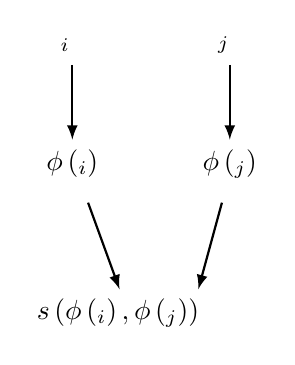
\begin{tikzpicture}[>=latex]
            \node[text width=0.5cm] at (2.1,5) {$\text{\PaperPortrait}_i$};
            \node[text width=0.5cm] at (4.1,5) {$\text{\PaperPortrait}_j$};

            \draw[->,thick] (2,4.75)--(2,3.8) node[below]{$\phi \left( \text{\PaperPortrait}_i \right)$};
            \draw[->,thick] (4,4.75)--(4,3.8) node[below]{$\phi \left( \text{\PaperPortrait}_j \right)$};

            \draw[->,thick] (2.2,3.0)--(2.6,1.9);
            \draw[->,thick] (3.9,3.0)--(3.6,1.9);

            \node[text width=0.5cm] at (1.8,1.6) {$s \left( \phi \left( \text{\PaperPortrait}_i \right), \phi \left( \text{\PaperPortrait}_j \right) \right)$};
        \end{tikzpicture}
        \begin{itemize}
            \item The function $s$ provides us with some notion of similarity between inputs after they've been "transformed" into a nicer form using a {\it feature map} $\phi$.
        \end{itemize}
    \end{figure}
\end{frame}

\section{Problem Significance}

\begin{frame}
    \frametitle{Problem Setting and Motivation}
    \begin{itemize}
        \item The idea of studying time series prediction came from a research group from the Gatton campus, lead by Dr Potgieter, analysing crop growth from previous seasons to forecast when certain phenological stages will take place in the current harvest.
    \end{itemize}
    \begin{figure}
        \centering
        \includegraphics[scale=0.18]{img/yan_wheat_GPR_plot.png}
    \end{figure}
\end{frame}

\section{Gaussian Processes}

\begin{frame}
    \frametitle{Introduction to Gaussian Processes}
    \begin{itemize}
        \item A Gaussian Process (GP) is a collection of random variables with index set $I$, such that every finite subset of random variables has a joint Gaussian distribution and are completely characterized by a mean function $m : X \to \mathbb{R}$ and a kernel $k : X \times X \to \mathbb{R}$ (in this context, think of the kernel as a function that provides some notion of similarity between points).
    \end{itemize}
    \begin{align*}
        m(\bm{x})           & = \mathbb{E} \left[ f(\bm{x}) \right]                                          \\
        k (\bm{x}, \bm{x'}) & = \mathbb{E} \left[ (f(\bm{x}) - m(\bm{x})) (f(\bm{x'}) - m(\bm{x'})) \right].
    \end{align*}
\end{frame}

\begin{frame}
    \frametitle{Predictions}
    \begin{itemize}
        \item Using the assumption that our data can be modelled as a Gaussian process, we can write out the new distribution of the observed noisy values along the points at which we wish to test the underlying function as
              \[
                  \begin{bmatrix}
                      \bm{y} \\
                      \bm{y}_{\star}
                  \end{bmatrix}
                  \sim \mathbb{N}
                  \begin{pmatrix}
                      \bm{0}, &
                      {
                              \begin{bmatrix}
                                  \bm{K_{XX}} + \sigma_n^2 \mathbb{I}_{n \times n} & \bm{K_{X_{\star}X}^{\intercal}} \\
                                  \bm{K_{X_{\star}X}}                              & \bm{K_{X_{\star}X_{\star}}}
                              \end{bmatrix}
                          }
                  \end{pmatrix}.
              \]
              (using the notation $\left( \bm{K}_{\bm{W} \bm{W}'} \right)_{i,j} \triangleq k \left( \bm{w}_i , \bm{w}_j' \right)$)
              \pause
        \item The mean and covariance can then be computed as
              \begin{align*}
                  \overline{\bm{y}_{\star}}           & = \bm{K_{X_{\star}X}} \left[ \bm{K_{XX}} + \sigma_n^2 \mathbb{I}_{n \times n} \right]^{-1} \bm{y}                                                         \\
                  \operatorname{cov} (\bm{y}_{\star}) & = \bm{K_{X_{\star}X_{\star}}} - \bm{K_{X_{\star}X}} \left[ \bm{K_{XX}} + \sigma_n^2 \mathbb{I}_{n \times n} \right]^{-1} \bm{K_{X_{\star}X}}^{\intercal}.
              \end{align*}
    \end{itemize}
\end{frame}

\begin{frame}
    \frametitle{Unoptimized GPR}
    {\centering
        \begin{minipage}{.9\linewidth}
            \begin{algorithm}[H]
                \caption{Unoptimized GPR}
                \SetAlgoLined
                \DontPrintSemicolon
                \SetKwInOut{Input}{input}\SetKwInOut{Output}{output}

                \Input{Observations $\bm{X}, \bm{y}$ and a test input $\bm{x}_{\star}$.}
                \Output{A prediction $\overline{f_{\star}} $ with its corresponding variance $ \mathbb{V} \left[ f_{\star} \right]$.}
                \BlankLine
                $\bm{L} = \operatorname{cholesky} \left( \bm{K_{XX}} + \sigma_n^2 \mathbb{I}_{n \times n} \right)$\;
                $\bm{\alpha} = \operatorname{lin-solve} \left( \bm{L}^{\intercal} , \operatorname{lin-solve} \left( \bm{L}, \bm{y} \right) \right)$\;
                $\overline{y_{\star}} = \bm{K_{x_{\star} X}} \bm{\alpha}$\;
                $\bm{v} = \operatorname{lin-solve} \left( \bm{L}, \bm{K_{x_{\star} X}} \right)$\;
                $\mathbb{V} \left[ f_{\star} \right] = \bm{K_{x_{\star} x_{\star}}} - \bm{v}^{\intercal} \bm{v}$\;
                \Return{$\overline{f_{\star}} , \mathbb{V} \left[ f_{\star} \right]$}
                \BlankLine
            \end{algorithm}
        \end{minipage}
        \par
    }
\end{frame}

\begin{frame}
    \frametitle{Problems with Unoptimized GPR}
    {\centering
        \begin{minipage}{.9\linewidth}
            \begin{algorithm}[H]
                \caption{Unoptimized GPR}
                \SetAlgoLined
                \DontPrintSemicolon
                \SetKwInOut{Input}{input}\SetKwInOut{Output}{output}

                \Input{Observations $\bm{X}, \bm{y}$ and a prediction inputs $\bm{x}_{\star}$.}
                \Output{A prediction $\overline{f_{\star}} $ with its corresponding variance $ \mathbb{V} \left[ f_{\star} \right]$.}
                \BlankLine
                \textcolor{red}{$\bm{L} = \operatorname{cholesky} \left( \bm{K_{XX}} + \sigma_n^2 \mathbb{I}_{n \times n} \right)$}\;
                \textcolor{red}{$\bm{\alpha} = \operatorname{lin-solve} \left( \bm{L}^{\intercal} , \operatorname{lin-solve} \left( \bm{L}, \bm{y} \right) \right)$}\;
                $\overline{f_{\star}} = \bm{K_{x_{\star} X}} \bm{\alpha}$\;
                \textcolor{red}{$\bm{v} = \operatorname{lin-solve} \left( \bm{L}, \bm{K_{x_{\star} X}} \right)$}\;
                $\mathbb{V} \left[ f_{\star} \right] = \bm{K_{x_{\star} x_{\star}}} - \bm{v}^{\intercal} \bm{v}$\;
                \Return{$\overline{f_{\star}} , \mathbb{V} \left[ f_{\star} \right]$}
                \BlankLine
            \end{algorithm}
        \end{minipage}
        \par
    }
    \begin{itemize}
        \item \textcolor{red}{Lines 1,2 and 4} can be incredibly slow as computing $\bm{K_{XX}}$ doing a Cholesky decomposition and performing linear solves scale poorly as the number of inputs, $n$, grows.
    \end{itemize}
\end{frame}

\section{Nystrom}

\begin{frame}
    \frametitle{Nystrom Approximation}
    \begin{itemize}
        \item The Nystrom method we seek a matrix $\bm{Q}\in \mathbb{R}^{n \times k}$ that satisfies $\norm{\bm{A} - \bm{Q} \bm{Q}^{\ast} \bm{A}}_{F} \leq \varepsilon$, where $\bm{A} \in \mathbb{R}^{n \times n}$ is positive semi definite matrix, to form the rank$-k$ approximation
              \begin{align*}
                  \onslide<1->{}
                  \onslide<2->{\bm{A} & \simeq \bm{Q} \bm{Q}^{\ast} \bm{A}                                                                                                                                \\}
                  \onslide<3->{       & \simeq \bm{Q} \left( \bm{Q}^{\ast} \bm{A} \bm{Q} \right) \bm{Q}^{\ast}                                                                                            \\}
                  \onslide<4->{       & = \bm{Q} \left( \bm{Q}^{\ast} \bm{A} \bm{Q} \right) \left( \bm{Q}^{\ast} \bm{A} \bm{Q} \right)^{\dagger} \left( \bm{Q}^{\ast} \bm{A} \bm{Q} \right) \bm{Q}^{\ast} \\}
                  \onslide<5->{       & \simeq \left( \bm{A} \bm{Q} \right) \left( \bm{Q}^{\ast} \bm{A} \bm{Q} \right)^{\dagger} \left( \bm{Q}^{\ast} \bm{A} \right).}
              \end{align*}
    \end{itemize}
\end{frame}

\section{Random Fourier Features}

\begin{frame}
    \frametitle{Random Fourier Feature Approximation}
    \begin{itemize}
        \item The RFF technique hinges on Bochners theorem which characterises positive definite functions (namely kernels) and states that any positive definite functions can be represented as
              \[
                  k \left( \bm{x}, \bm{y} \right) = k \left( \bm{x} - \bm{y} \right) = \int_{\mathbb{C}^d} \exp \left( i \langle \bm{\omega} , \bm{x} - \bm{y} \rangle \right) \mu_k \left( d \bm{\omega} \right)
              \]
              where $\mu_k$ is a positive finite measure on the frequencies of $\bm{\omega}$.
              \pause
        \item This integral can then be approximated via the following Monte Carlo estimate
              \begin{align*}
                  \onslide<1->{}
                  \onslide<2->{k \left( \bm{x} - \bm{y} \right)
                                & = \int_{\mathbb{C}^d} \exp \left( i \langle \bm{\omega} , \bm{x} - \bm{y} \rangle \right) p (\bm{\omega}) \; d \bm{\omega}                                                                                                     \\}
                  \onslide<3->{ & = \mathbb{E}_{\bm{\omega} \sim p (\cdot)} \left( \exp \left( i \langle \bm{\omega} , \bm{x} - \bm{y} \rangle \right) \right)                                                                                                   \\}
                  \onslide<4->{ & \simeq \frac{1}{D} \sum_{j=1}^{D} \exp \left( i \langle \bm{\omega}_{j} , \bm{x} - \bm{y} \rangle \right)                                                                                                                      \\}
                  \onslide<5->{ & = \sum_{j=1}^{D} \left( \frac{1}{\sqrt{D}} \exp \left( i \langle \bm{\omega}_{j} , \bm{x} \rangle \right) \right) \overline{\left( \frac{1}{\sqrt{D}} \exp \left( i \langle \bm{\omega}_{j} , \bm{y} \rangle \right) \right) } \\}
                  \onslide<6->{ & = \langle \varphi (\bm{x}) , \varphi (\bm{y}) \rangle_{\mathbb{C}^D}}
              \end{align*}
    \end{itemize}
\end{frame}

\section{Results}

\begin{frame}
    \begin{figure}
        \centering
        \subfloat[3D-Spatial network]{
            \begin{adjustbox}{width=0.31\textwidth}
                \includegraphics[scale=1]{img/results/nys-sigma=0.1-k=80.png}
            \end{adjustbox}
        }
        \subfloat[Abalone]{
            \begin{adjustbox}{width=0.31\textwidth}
                \includegraphics[scale=1]{img/results/nys-sigma=1.0-k=20.png}
            \end{adjustbox}
        }
        \subfloat[Temperature]{
            \begin{adjustbox}{width=0.31\textwidth}
                \includegraphics[scale=1]{img/results/nys-sigma=1.0-k=80.png}
            \end{adjustbox}
        }
        \caption{Comparison of Nystrom methods for various datasets.}
    \end{figure}
    \begin{figure}
        \centering
        \subfloat[3D-Spatial network]{
            \begin{adjustbox}{width=0.31\textwidth}
                \includegraphics[scale=1]{img/results/rff-sigma=0.1.png}
            \end{adjustbox}
        }
        \subfloat[Abalone]{
            \begin{adjustbox}{width=0.31\textwidth}
                \includegraphics[scale=1]{img/results/rff-sigma=10.0.png}
            \end{adjustbox}
        }
        \subfloat[Wine]{
            \begin{adjustbox}{width=0.31\textwidth}
                \includegraphics[scale=1]{img/results/rff-sigma=2.1.png}
            \end{adjustbox}
        }
        \caption{Comparison of RFF methods for various datasets.}
    \end{figure}
\end{frame}

\begin{frame}
    \begin{figure}
        \centering
        \subfloat[Frobenius error]{
            \begin{adjustbox}{width=0.45\textwidth}
                \includegraphics[scale=1]{img/results/cmp_rel-sigma=0.1-k=80.png}
            \end{adjustbox}
        }
        \subfloat[Infinity error]{
            \begin{adjustbox}{width=0.45\textwidth}
                \includegraphics[scale=1]{img/results/cmp_inf-sigma=0.1-k=80.png}
            \end{adjustbox}
        }
        \caption{Comparison between Nystrom and RFF approximations for the 3D-Spatial network data.}
    \end{figure}
\end{frame}

\section{Moving Forward}

\begin{frame}
    \frametitle{Moving Forward}
    \begin{itemize}
        \item We saw that the Nystrom technique is better at producing approximations of the Gram matrix, $\bm{K}_{\bm{XX}}$, with smaller {\it relative Frobenius errors} while the RFF technique is better at producing approximations with smaller {\it relative infinity errors}. Which is better for GP prediction?
        \item Recall, the other bottle neck in the GPR algorithm was the Cholesky decomposition. We can employ faster linear system solvers, namely the {\it Conjugate Gradient} (CG) and {\it Minimum Residual} (MINRES) method.
    \end{itemize}
\end{frame}

\end{document}